
Valgrind (\url{https://www.valgrind.org})是一个工具框架,允许构建动态分析实用程序——在运行时进行分析。提供了很多工具套件,允许进行各种调查和检查。其中一些工具如下:

\begin{itemize}
\item 
Memcheck – 检测内存管理问题

\item 
Cachegrind – 配置CPU缓存,并指出缓存缺失和其他缓存问题

\item 
Callgrind – Cachegrind的扩展,提供了调用图的信息

\item 
Massif – 堆分析器,显示程序的哪些部分在特定时段内使用堆

\item 
Helgrind – 线程调试器,帮助解决数据竞争问题

\item 
DRD – 更轻的限量版Helgrind
\end{itemize}

列表中的每一个工具都非常方便。大多数包管理器都知道Valgrind,并且可以轻松地将它安装到操作系统上(若使用的是Linux,可能已经安装了它)。并且,官方网站提供了源代码,也可以自己构建。

我们将把重点限制在套件中最有用的应用程序上。当提到Valgrind时,通常指的是Valgrind的Memcheck。让我们了解一下如何在CMake中使用它——这将为使用其他工具铺平道路。

\subsubsubsection{9.4.1\hspace{0.2cm}Memcheck}

调试内存问题时,Memcheck不可缺少。开发者对如何管理内存有很大的控制权,所以这个主题在C++中特别棘手。各种各样的错误都有可能发生:读取未分配的内存、读取已经释放的内存、多次尝试释放内存,以及写入不正确的地址。开发人员显然试图避免这些错误,但由于这些错误不显眼,甚至可以潜入最简单的程序。有时,只要一个遗忘的变量初始化,就会我们让陷入困境。

使用Memcheck的方式是这样的:

\begin{tcblisting}{commandshell={}}
valgrind [valgrind-options] tested-binary [binary-options]
\end{tcblisting}

Memcheck是Valgrind的默认工具,也可以显式选择它:

\begin{tcblisting}{commandshell={}}
valgrind --tool=memcheck tested-binary
\end{tcblisting}

运行Memcheck的开销很大。手册(参见扩展阅读中的链接)里说,它可使程序慢10-15倍。为了避免每次运行测试时都等待Valgrind,可以创建一个单独的目标,在需要测试代码时从命令行调用该目标。理想情况下,开发人员将在将更改合并到存储库的默认分支之前运行。这可以通过Git钩子完成,也可以作为CI流水中的一个步骤。要构建一个自定义目标,需要在生成阶段完成后使用以下命令:

\begin{tcblisting}{commandshell={}}
cmake --build <build-tree> -t valgrind
\end{tcblisting}

添加这样一个目标并不难:

\begin{lstlisting}[style=styleCMake]
# chapter09/03-valgrind/cmake/Valgrind.cmake

function(AddValgrind target)
	find_program(VALGRIND_PATH valgrind REQUIRED)
	add_custom_target(valgrind
		COMMAND ${VALGRIND_PATH} --leak-check=yes
			$<TARGET_FILE:${target}>
		WORKING_DIRECTORY ${CMAKE_BINARY_DIR}
	)
endfunction()
\end{lstlisting}

本例中,创建了一个CMake模块(因此我们可以跨项目重用相同的文件)包装函数,将接受要测试的目标。这里会发生两件事:

\begin{itemize}
\item 
CMake搜索valgrind可执行文件的默认系统路径,并将其存储在VALGRIND\_PATH变量中。若没有找到二进制文件,REQUIRED关键字将停止配置并报错。

\item 
创建了一个自定义目标valgrind,将在目标二进制文件上执行Memcheck工具,这里还添加了一个检查内存泄漏的选项。
\end{itemize}

当涉及到Valgrind选项时,可以作为命令行参数提供,也可以使用以下方式提供:

\begin{enumerate}
\item 
~/.valgrindrc文件(在主目录中)

\item 
\$VALGRIND\_OPTS环境变量

\item 
./.Valgrindrc文件(在工作目录中)
\end{enumerate}

这些是按顺序检查的。另外,最后一个文件只有在属于当前用户、是常规文件且没有标记为全球可写的情况下才会考虑。因为给Valgrind的选项可能是潜在有害,所以这是一种安全的机制。

要使用AddValgrind函数,应该为它提供一个unit\_tests目标:

\begin{lstlisting}[style=styleCMake]
# chapter09/03-valgrind/test/CMakeLists.txt (fragment)

# ...
add_executable(unit_tests calc_test.cpp run_test.cpp)
# ...
include(Valgrind)
AddValgrind(unit_tests)
\end{lstlisting}

使用Debug配置生成构建树允许Valgrind进入调试信息,这使它的输出更加清晰。来看看在实践中是如何工作的:

\begin{tcblisting}{commandshell={}}
# cmake --build <build-tree> -t valgrind
\end{tcblisting}

这将构建sut和unit\_tests目标:

\begin{tcblisting}{commandshell={}}
[100%] Built target unit_tests
\end{tcblisting}

开始执行Memcheck,其为提供了基本信息:

\begin{tcblisting}{commandshell={}}
==954== Memcheck, a memory error detector
==954== Copyright (C) 2002-2017, and GNU GPL'd, by Julian
Seward et al.
==954== Using Valgrind-3.15.0 and LibVEX; rerun with -h for
copyright info
==954== Command: ./unit_tests
\end{tcblisting}

前缀==954==包含进程ID。添加这一点是为了将Valgrind注释与测试过程的输出区分开来。

接下来,使用gtest运行测试:

\begin{tcblisting}{commandshell={}}
[==========] Running 3 tests from 2 test suites.
[----------] Global test environment set-up.
...
[==========] 3 tests from 2 test suites ran. (42 ms total)
[ PASSED ] 3 tests.
\end{tcblisting}

最后,进行总结:

\begin{tcblisting}{commandshell={}}
==954==
==954== HEAP SUMMARY:
==954== in use at exit: 1 bytes in 1 blocks
==954== total heap usage: 209 allocs, 208 frees, 115,555
bytes allocated
\end{tcblisting}

啊哦!我们仍然使用至少1个字节。使用malloc()和new进行的分配与适当的free()和delete操作不匹配,程序似乎有内存泄漏。Valgrind提供了更多的细节来找到它:

\begin{tcblisting}{commandshell={}}
==954== 1 bytes in 1 blocks are definitely lost in loss record
1 of 1
==954== at 0x483BE63: operator new(unsigned long) (in /usr/
lib/x86_64-linux-gnu/valgrind/vgpreload_memcheck-amd64-linux.
so)
==954== by 0x114FC5: run() (run.cpp:6)
==954== by 0x1142B9: RunTest_RunOutputsCorrectEquations_
Test::TestBody() (run_test.cpp:14)
\end{tcblisting}

以by 0x<address>开头的行表示调用堆栈中的各个函数。这里截断了输出(有一些输出来自GTest),以关注有趣的部分——最顶层的函数和源引用,run()(run.cpp:6):最后,在底部找到总结信息:

\begin{tcblisting}{commandshell={}}
==954== LEAK SUMMARY:
==954==     definitely lost: 1 bytes in 1 blocks
==954==     indirectly lost: 0 bytes in 0 blocks
==954==       possibly lost: 0 bytes in 0 blocks
==954==     still reachable: 0 bytes in 0 blocks
==954==          suppressed: 0 bytes in 0 blocks
==954==
==954== ERROR SUMMARY: 1 errors from 1 contexts (suppressed: 0
from 0)
\end{tcblisting}

Valgrind在发现非常复杂的问题方面做得很好,还能够更深入地挖掘,找到无法自动分类的可疑情况。这些发现将归入可能丢失的那一类。

来看看Memcheck在这个案例中发现了什么问题:

\begin{lstlisting}[style=styleCXX]
// chapter09/03-valgrind/src/run.cpp

#include <iostream>
#include "calc.h"
using namespace std;

int run() {
	auto c = new Calc(); // ERROR
	cout << "2 + 2 = " << c->Sum(2, 2) << endl;
	cout << "3 * 3 = " << c->Multiply(3, 3) << endl;
	return 0;
}
\end{lstlisting}

没错:突出显示的代码是错误的。事实上,我们确实创建了一个在测试结束之前没有删除的对象。这就是为什么拥有广泛的测试覆盖率是如此重要的确切原因。

Valgrind是一个非常有用的工具,但是在处理更复杂的程序时,其输出会变得有点冗长。必须有一种方法,以更易于管理的形式收集这些信息。

\subsubsubsection{9.4.2\hspace{0.2cm}Memcheck-Cover}

商业IDE(如CLion)本身支持将Valgrind的输出解析为可以在GUI中轻松导航的内容,而无需通过控制台窗口滚动来查找正确的消息。若编辑器没有这个选项,可以通过使用第三方报告生成器更清楚地查看错误。David Garcin编写的Memcheck-cover以生成HTML文件的形式提供了更好的体验,如图9.1所示:

\begin{center}
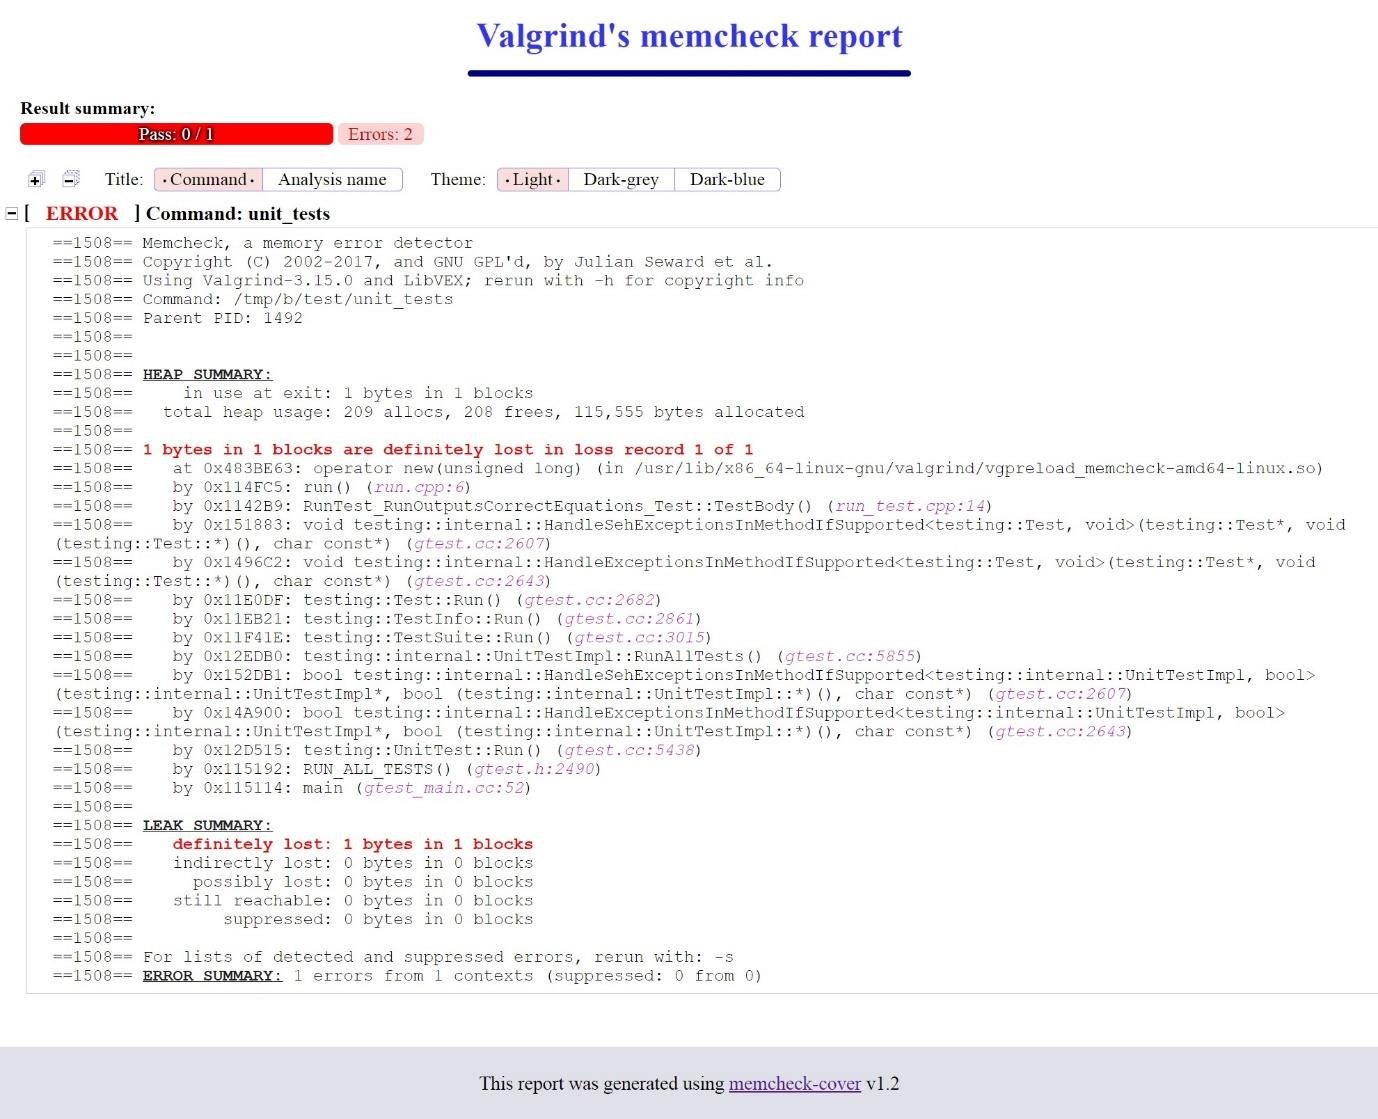
\includegraphics[width=0.8\textwidth]{content/3/chapter9/images/1.jpg}\\
图9.1 由memcheck-cover生成的报告
\end{center}

这个整洁的小项目可以在GitHub(\url{https://github.com/Farigh/memcheck-cover})上找到,需要Valgrind和gawk (GNU AWK工具)。要使用它,需要在单独的CMake模块中准备一个setup函数。其由两部分组成:

\begin{itemize}
\item 
获取和配置工具

\item 
添加执行Valgrind并生成报告的自定义目标
\end{itemize}

配置如下所示:

\begin{lstlisting}[style=styleCMake]
# chapter09/04-memcheck/cmake/Memcheck.cmake

function(AddMemcheck target)
	include(FetchContent)
	FetchContent_Declare(
	memcheck-cover
		GIT_REPOSITORY https://github.com/Farigh/memcheckcover.git
		GIT_TAG release-1.2
	)
	FetchContent_MakeAvailable(memcheck-cover)
set(MEMCHECK_PATH ${memcheck-cover_SOURCE_DIR}/bin)
\end{lstlisting}

第一部分中,我们遵循与常规依赖项相同的实践:包括FetchContent模块,并使用FetchContent\_Declare指定项目的存储库和所需的Git标记。接下来,启动获取过程,并使用FetchContent\_Populate(由FetchContent\_MakeAvailable隐式调用)设置的memcheck-cover\_SOURCE\_DIR变量配置到二进制文件的路径。

该函数的第二部分是创建生成报告的目标,将其命名为memcheck(这样就不会与之前的valgrind目标重叠):

\begin{lstlisting}[style=styleCMake]
# chapter09/04-memcheck/cmake/Memcheck.cmake (continued)

	add_custom_target(memcheck
		COMMAND ${MEMCHECK_PATH}/memcheck_runner.sh -o
			"${CMAKE_BINARY_DIR}/valgrind/report"
			-- $<TARGET_FILE:${target}>
		COMMAND ${MEMCHECK_PATH}/generate_html_report.sh
			-i "${CMAKE_BINARY_DIR}/valgrind"
			-o "${CMAKE_BINARY_DIR}/valgrind"
		WORKING_DIRECTORY ${CMAKE_BINARY_DIR}
	)
endfunction()
\end{lstlisting}

这发生在两个命令中:

\begin{enumerate}
\item 
首先,运行memcheck\_runner.sh包装器脚本,该脚本将执行Valgrind的memcheck并将输出收集到带有-o参数的文件中。

\item 
然后,将解析输出并使用generate\_html\_report.sh创建报告。这个脚本需要使用-i和-o参数提供的输入和输出目录。
\end{enumerate}

两个步骤都应该在CMAKE\_BINARY\_DIR工作目录中执行,以便单元测试二进制在需要时通过相对路径访问文件。

需要添加到列表文件的最后一件事当然是对这个函数的调用,与AddValgrind有相同的模式:

\begin{lstlisting}[style=styleCMake]
# chapter09/04-memcheck/test/CMakeLists.txt (fragment)

include(Memcheck)
AddMemcheck(unit_tests)
\end{lstlisting}

用Debug配置生成一个构建系统之后,可以用以下方法构建目标:

\begin{tcblisting}{commandshell={}}
cmake --build <build-tree> -t memcheck
\end{tcblisting}

然后,就可以享受格式化的报告了。为了真正享受它,需要在run.cpp中添加缺失的delete c;,使它停止抱怨(或者,使用智能指针)。








